\chapter{Introduction}\label{ch:introduction}

In this work we explored the ability of screening for (type 2) diabetes mellitus based on Belgian health insurance data from a machine learning perspective. The thesis is organized as a collection of papers concerning various aspects related to this application. This chapter provides some context of the project, both in terms of the medical situation and the challenges in terms of data analysis. 

This work aligns with the overall trend towards eHealth and the rising use of all sorts of data for evidence-based medicine. However, relevant policies are still in flux, specifically those related to the use of patient records vis-\`a-vis privacy. The key novelty of this work -- the effective use of health expenditure data for clinical applications -- adds another dimension to this important ongoing debate.

We will first briefly introduce diabetes mellitus and describe the main characteristics of the disease, its treatment and existing screening approaches in Section~\ref{intro:diabetes}. The Belgian health insurance landscape is described in Section~\ref{intro:health-insurance}. Subsequently, Section~\ref{intro:machine-learning} contains a discussion of the main challenges of this project from a machine learning perspective to explain the necessity of each aspect of our research. Finally, Section~\ref{intro:structure} summarizes the structure of the text and indicates how all chapters (papers) are related to each other.

%\instructionsintroduction

%%%%%%%%%%%%%%%%%%%%%%%%%%%%%%%%%%%%%%%%%%%%%%%%%%%
%               DIABETES
%%%%%%%%%%%%%%%%%%%%%%%%%%%%%%%%%%%%%%%%%%%%%%%%%%%

\section{Diabetes mellitus} \label{intro:diabetes}
Diabetes mellitus is a metabolic disorder characterized by chronic hyperglycemia, which is primarily caused by insufficient insulin secretion and/or insulin resistance \citep{alberti1998definition}. The worldwide incidence of diabetes has increased dramatically over the last century due to changes in human behaviour and lifestyle \citep{zimmet2001global, chen2012worldwide}. Diabetes is one of the main threats to human health world wide \citep{king1998global, zimmet2001global, zimmet2000globalization} and is projected to be the 7th leading cause of death by 2030 \citep{mathers2006projections}. Some key facts related to diabetes mellitus are summarized in the diabetes atlas made by the International Diabetes Federation (IDF) (Figure~\ref{intro:diabetes-infogram}).


In the remainder of this Section we provide a brief overview of various aspects of the disease: the underlying biological problem, common complications and comorbidities, a classification of diabetes based on etiology, the prevalence and burden of the disorder and finally treatment and existing screening approaches.

\begin{figure}[p]
  \centering
  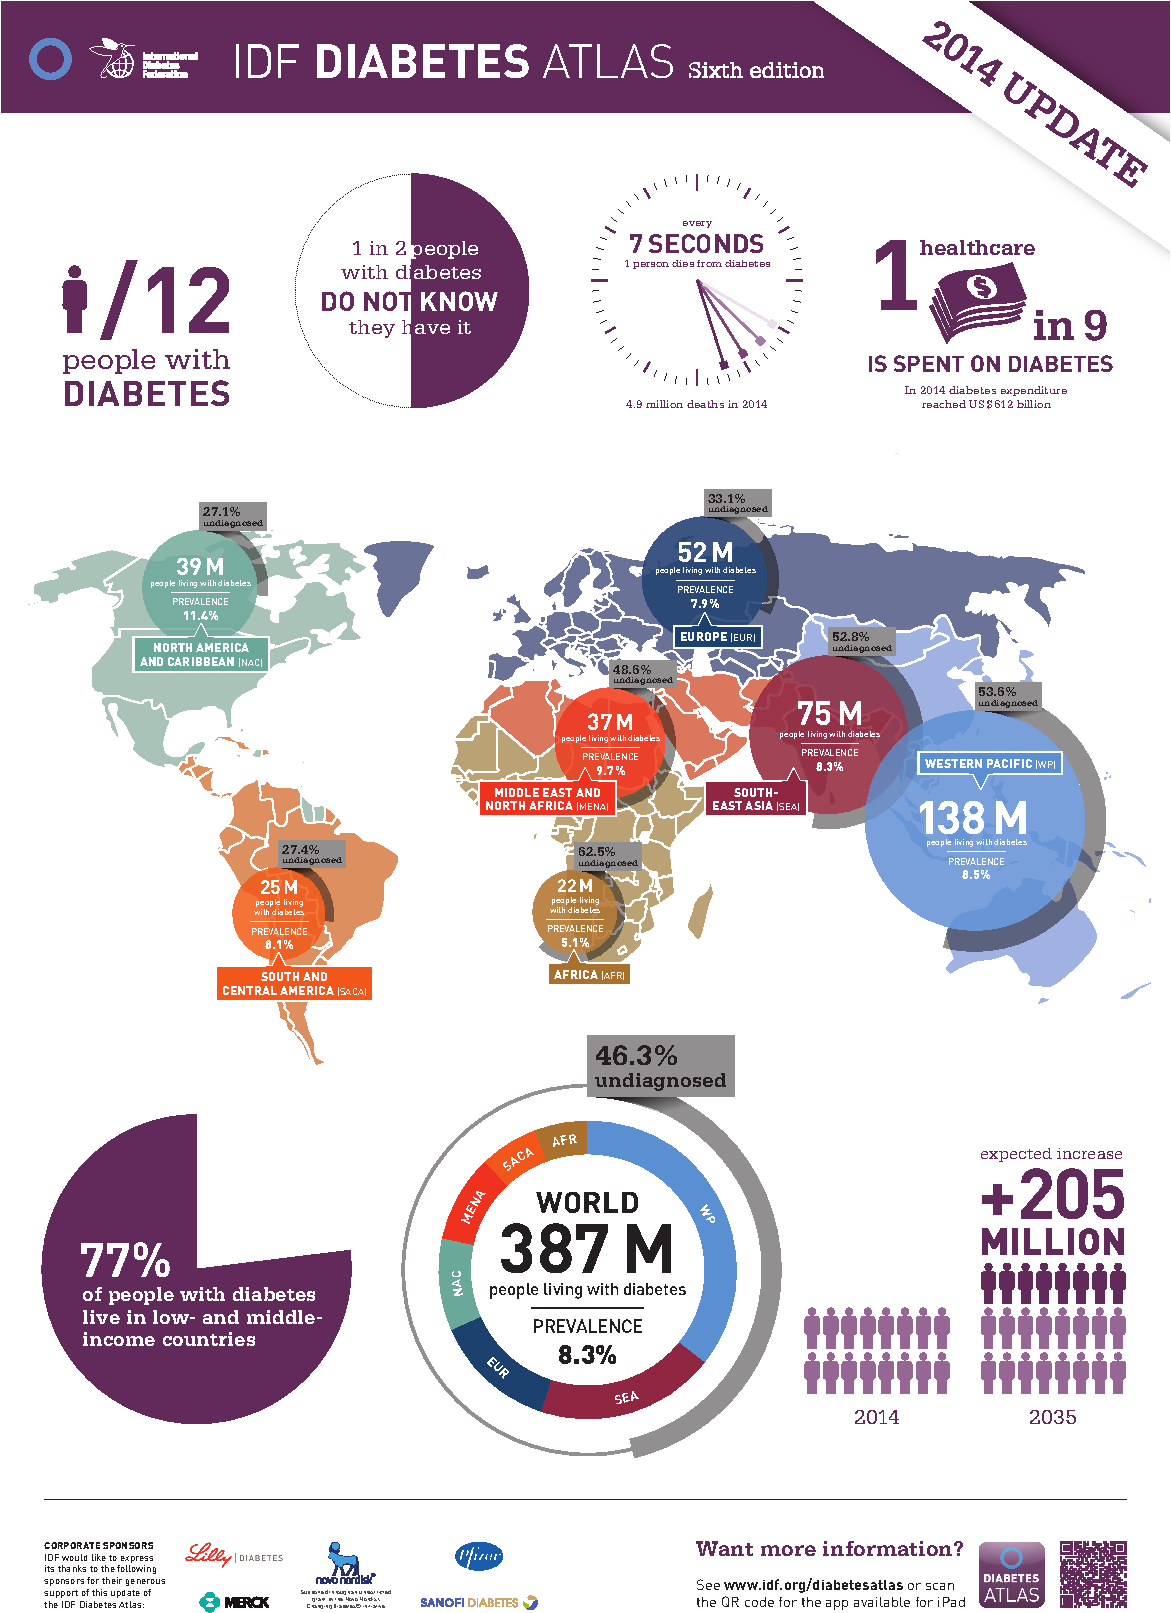
\includegraphics[width=\textwidth]{infogram-cropped.pdf}
  \caption{Diabetes atlas released by the International Diabetes Federation (IDF). Reuse of this material was granted by the IDF. The original is available at \url{http://www.idf.org/worlddiabetesday/toolkit/gp/facts-figures}.} 
  \label{intro:diabetes-infogram}
\end{figure}


%%%%%%%%%%%%%%%%%%%%%%%%%%%%%%%%%%%%%%%%%%%%%%%%
%      REGULATION OF BLOOD GLUCOSE LEVEL       %
%%%%%%%%%%%%%%%%%%%%%%%%%%%%%%%%%%%%%%%%%%%%%%%%

\subsection{Regulation of blood glucose levels}
To allow a better understanding of the underlying problems inherent to diabetes mellitus, we will briefly describe the critical role of insulin in the regulation of blood glucose levels.

Insulin is a peptide hormone which regulates the metabolism of fats and carbohydrates. In normal circumstances, insulin is released in response to changes in blood glucose concentration to prevent glucose levels from reaching toxic concentrations. Specifically, insulin promotes the absorption of glucose from the blood to skeletal muscles and fat tissue, thereby lowering the glucose level in the bloodstream, and additionally inhibits hepatic glucose output \citep{sonksen2000insulin}. Insulin is exclusively produced by pancreatic $\beta$ cells, which are located in clusters known as the islets of Langerhans. 

Hyperglycemia occurs when the regulation of the blood glucose level fails and hence toxic concentrations of glucose remain in the bloodstream. Such failures are typically caused by excessive glucose intake, insufficient insulin secretion and/or insulin resistance. 

%%%%%%%%%%%%%%%%%%%%%%%%%%%%%%%%%%%%%%%%%%%%%%%%
%         COMPLICATIONS AND COMORBIDITIES      %
%%%%%%%%%%%%%%%%%%%%%%%%%%%%%%%%%%%%%%%%%%%%%%%%

\subsection{Complications and comorbidities}
Exposure to chronic hyperglycemia can cause serious damage to many of the body's systems, including dysfunction and failure of various organs.

The leading complication of type 2 diabetes is cardiovascular disease, with about half of type 2 diabetes patient deaths attributable to a cardiovascular cause \citep{doi:10.1001/jama.2009.476, beulens2010global}. Microvascular complications also contribute considerably to the morbidity of the disease, specifically diabetes mellitus may lead to the progressive development of retinopathy (which potentially results in blindless), neuropathy (which can induce problems like foot ulcers), nephropathy (which can lead to renal failure) \citep{atkins2010diabetic} and small vessel vasculopathy causing lower extremity amputation \citep{beulens2010global}. Finally, patients with diabetes mellitus are at increased risk for peripheral vascular and cerebrovascular disease. 


% The global burden of diabetes and its complications: an emerging pandemic
% Cardiovascular disease (CVD) is the leading complication of type 2 diabetes and approximately one half of patients with type 2 diabetes will die of a cardiovascular cause. Angina, myocardial infarction, stroke, peripheral artery disease, and congestive heart failure are all common among patients with type 2 diabetes. IFG or IGT and the risks are further compounded by smoking, abnormal blood lipids, high blood pressure, and the other determinants of vascular risk established in nondiabetic populations [1,18].


% http://www.who.int/mediacentre/factsheets/fs312/en/
% What are common consequences of diabetes?
% Over time, diabetes can damage the heart, blood vessels, eyes, kidneys, and nerves.
% Diabetes increases the risk of heart disease and stroke. In a multinational study, 50% of people with diabetes die of cardiovascular disease (primarily heart disease and stroke) (6). Combined with reduced blood flow, neuropathy (nerve damage) in the feet increases the chance of foot ulcers, infection and eventual need for limb amputation. Diabetic retinopathy is an important cause of blindness, and occurs as a result of long-term accumulated damage to the small blood vessels in the retina. One percent of global blindness can be attributed to diabetes (7). Diabetes is among the leading causes of kidney failure (4). The overall risk of dying among people with diabetes is at least double the risk of their peers without diabetes (8).
% (2) World Health Organization. Global Health Estimates: Deaths by Cause, Age, Sex and Country, 2000-2012. Geneva, WHO, 2014. 
% (3) Mathers CD, Loncar D. Projections of global mortality and burden of disease from 2002 to 2030. PLoS Med, 2006, 3(11):e442.
% (4) Global status report on noncommunicable diseases 2010. Geneva, World Health Organization, 2011. 
% (5) Definition, diagnosis and classification of diabetes mellitus and its complications. Part 1: Diagnosis and classification of diabetes mellitus. Geneva, World Health Organization, 1999 (WHO/NCD/NCS/99.2). 
% (6) Morrish NJ, Wang SL, Stevens LK, Fuller JH, Keen H. Mortality and causes of death in the WHO Multinational Study of Vascular Disease in Diabetes. Diabetologia 2001, 44 Suppl 2:S14–S21.
% (7) Global data on visual impairments 2010. Geneva, World Health Organization, 2012.
% (8) Roglic G, Unwin N, Bennett PH, Mathers C, Tuomilehto J, Nag S et al. The burden of mortality attributable to diabetes: realistic estimates for the year 2000. Diabetes Care, 2005, 28(9):2130–2135.

%%%%%%%%%%%%%%%%%%%%%%%%%%%%%%%%%%%%%%%%%%%%%%%%%
%         CLASSIFICATION OF DIABETES            %
%%%%%%%%%%%%%%%%%%%%%%%%%%%%%%%%%%%%%%%%%%%%%%%%%

\subsection{Classification of diabetes mellitus}

Diabetes mellitus is a disorder of multiple etiologies and is subdivided into several more specific classes. The primary distinction between subclasses is essentially whether or not external insulin is necessary for survival. The first widely accepted classification was made by the World Health Organization (WHO) in 1980 \citep{WHO1980}, proposing two main classes of diabetes mellitus:
\begin{itemize}
\item \textbf{Type 1 diabetes (T1D)} refers to a condition characterized by insufficient insulin secretion caused by the autoimmune-mediated destruction of pancreatic $\beta$-cells. T1D patients require insulin for survival. T1D can start at an early age and has a strong genetic component.
\item \textbf{Type 2 diabetes (T2D)} results from defect(s) in insulin secretion, almost always paired with insulin resistance. T2D includes patients that require insulin for metabolic control and those that don't require insulin at all. The often asymptomatic onset of T2D typically occurs after 50 years of age\footnote{Though a case-study reported a 3 year-old child diagnosed with T2D at this year's European Association for the Study of Diabetes (EASD) meeting \citep[``\emph{A toddler with type 2 diabetes}'', pp. 152--153]{3yeardolddiabetic}.} and is often a result of genetic susceptibility combined with chronic obesity, a sedentary lifestyle and overly rich nutrition \citep{zimmet2001global, smyth2006diabetes}. Since obesity is such a common comorbidity of T2D \citep{smyth2006diabetes}, the terms \emph{diabesity} and \emph{obesity dependent diabetes mellitus} have been suggested \citep{shafrir1996development, astrup2000redefining}.
\end{itemize}
In the original proposal, T1D and T2D were aliased insulin-dependent diabetes mellitus (IDDM) and noninsulin-dependent diabetes mellitus (NIDDM), respectively \citep{WHO1980}. However, since then the WHO has deprecated the terms IDDM and NIDDM as their use frequently led to patients being classified based on treatment, rather than pathogenesis \citep{alberti1998definition}. Hence, contemporary terminology exclusively uses type 1 and type 2 to denote the main classes of diabetes mellitus. 

Though our work focuses on type 1 and particularly type 2 diabetes mellitus, it must be noted that more forms exist, such as gestational diabetes mellitus which may occur during pregnancy and then disappear or progress into T2D.

T2D accounts for over $90\%$ of diabetes patients and has long been considered an epidemic that affects both developing and developed nations \citep{zimmet1999diabetes,zimmet2001global,rocchini2002childhood,nathan2007impaired,chen2012worldwide, lam2012worldwide} effectively rendering it a pandemic \citep{beulens2010global}. T2D is often a manifestation of a much broader underlying disorder \citep{reaven1988role, zimmet1999diabetes}, including the \emph{metabolic syndrome} which is a cluster of cardiovascular disease risk factors that includes hyperinsulinemia, dislipidemia, hypertension, visceral obesity, hypercoagulability and microalbuminuria \citep{alberti2005metabolic, zimmet2001global, federation2010idf}. 

%%%%%%%%%%%%%%%%%%%%%%%%%%%%%%%%%%%%%%%%%%%%
%         PREVALENCE AND BURDEN            %
%%%%%%%%%%%%%%%%%%%%%%%%%%%%%%%%%%%%%%%%%%%%

\subsection{Prevalence and burden of diabetes}
The number of diabetes patients, particularly type 2 diabetes, is increasing rapidly. In developed countries, this increase is driven by population aging, lifestyle changes (particularly rising levels of obesity and inactivity) but also by greater longevity among diabetes patients \citep{stovring2003rising,beulens2010global}. The majority of social and economic burden of type 2 diabetes patients is attributable to vascular complications \citep{beulens2010global}, with pharmacy costs generating the majority of diabetes-related health expenditure \citep{nichols2002impact, gandra2006total}.

\paragraph{Prevalence} In 1995 an estimated 135 million people worldwide had diabetes, which has increased to 285 million patients worldwide in 2010 \citep{shaw2010global, chen2012worldwide} and is predicted by the WHO to increase further to at least 366 million by 2030 \citep{smyth2006diabetes}. WHO estimated the global prevalence of diabetes to be $9\%$ among adults over 18 years of age \citep{alwan2011global}. A recent study estimated the prevalence of diabetes in adults aged 20--79 in Belgium and Europe to be $8\%$ and $6.9\%$, respectively \citep{shaw2010global}. Typically, the prevalence of prediabetes is estimated even higher \citep{cowie2009full,yang2010prevalence,chen2012worldwide}.

\paragraph{Mortality} 
The premature mortality attributable to diabetes is widely underestimated because only a minority of persons with diabetes die from a cause that is uniquely attributable to diabetes \citep{beulens2010global}. A study reported about 2.9 million deaths worldwide attributable to diabetes \citep{roglic2005burden}. The same study indicates that this excess mortality accounts for over $8\%$ of deaths in developed countries. More recently, the global excess mortality in adults directly related to diabetes has been estimated to 3.8 million deaths \citep{beulens2010global}. The main causes of premature deaths in type 2 diabetes patients are due to cardiovascular and renal problems \citep{morrish2001mortality, beulens2010global}. 
Chapter~\ref{ch:survival} reports the survival of patients starting various glucose lowering pharmacotherapies in Belgium and confirms excess mortality in patients with diabetes compared to the general population. Additionally, our analysis indicates that the excess mortality depends significantly on the type of pharmacotherapy, which is related to the patient's health status.


\paragraph{Cost} Managing diabetes and its complications is expensive, both to the affected individuals and healthcare systems around the world.  The International Diabetes Federation (IDF), estimates that diabetes already accounts for one ninth of the total healthcare budget in many countries in 2014 \citep{IDFfacts}. The IDF further reports an average cost per diabetes patient of 5,679 USD in Belgium \citep{IDFatlas}. Other sources report comparable numbers: the CoDiM study estimated that in Germany in 2001, annual direct mean costs per diabetic patient are $5,262$ EUR with an additional $5,019$ EUR indirect costs, compared to $2,755$ EUR and $3,691$ EUR for non-diabetics \citep{koster2006cost}. K\"oster et al. \citep{koster2006cost} also note that the direct costs of diabetic patients account for $14.2\%$ of total healthcare costs. Patients of type 2 diabetes with macrovascular complications generate costs that are three times higher than type 2 diabetes patients without macrovascular complications and seven times higher than people with neither type 2 diabetes nor macrovascular diseases \citep{beulens2010global}. The primary origin of diabetes-related healthcare expenditure are pharmacy costs \citep{nichols2002impact, gandra2006total}. The complications of diabetes constitute a large portion of the burden of the disease, with diabetes being a leading cause of blindness, lower limb amputation and kidney failure \citep{beulens2010global}. 


% http://europepmc.org/abstract/med/18350480
% http://download.springer.com/static/pdf/651/art%253A10.1007%252Fs00125-002-0860-3.pdf?originUrl=http%3A%2F%2Flink.springer.com%2Farticle%2F10.1007%2Fs00125-002-0860-3&token2=exp=1440768601~acl=%2Fstatic%2Fpdf%2F651%2Fart%25253A10.1007%25252Fs00125-002-0860-3.pdf%3ForiginUrl%3Dhttp%253A%252F%252Flink.springer.com%252Farticle%252F10.1007%252Fs00125-002-0860-3*~hmac=7111eff228db17edf0730fb32261e2f1d4a0400afbf88526eaa03e1bf6fe3f23
% http://informahealthcare.com/doi/abs/10.1185/030079905x65349
% http://cpr.sagepub.com/content/17/1_suppl/s3.full



\subsection{Treatment of diabetes mellitus} \label{intro:treatment}
%%%%%%%%%%%%%%%%%%%%%%%%%%%%%%%%%%%%
%%%%%%%%%%%%%%%%%%%%%%%%%%%%%%%%%%%%
%%%%%%%%%%%%%%%%%%%%%%%%%%%%%%%%%%%%
%%%%%%%v TODO   %%%%%%%%%%%%%%%%%%%%
%%%%%%%%%%%%%%%%%%%%%%%%%%%%%%%%%%%%
%%%%%%%%%%%%%%%%%%%%%%%%%%%%%%%%%%%%
%%%%%%%%%%%%%%%%%%%%%%%%%%%%%%%%%%%%
%%%%%%%%%%%%%%%%%%%%%%%%%%%%%%%%%%%%
%\todo{TODO prevention of complications http://www.nature.com/nature/journal/v414/n6865/full/414782a.html}
The fact chronic hyperglycemia may manifest in various ways is reflected in a wide variety of treatments for diabetes mellitus. Treatment of type 1 diabetes patients revolves around timely administration of external insulin, which they need for survival. In contrast, a wide range of treatment options exist for patients with type 2 diabetes.

Management of type 2 diabetes includes several lifestyle interventions, often specifically targetted towards weight loss, including healthy eating (specifically high-fiber, low-fat foods like fruits and vegetables), regular exercise and blood sugar monitoring and management. Pharmacotherapy via glucose lowering agents (GLAs) is used when lifestyle changes alone are insufficient for adequate glycemic control or when diabetes is already in a progressed stage at the time of clinical diagnosis. 

We will elaborate on pharmacological treatment of type 2 diabetes, as this has played a crucial role in our work. Pharmacological therapies for (type 2) diabetes may be based on various biological mechanisms:
\begin{itemize}
\item \textbf{External insulin} is administered when insufficient insulin is secreted by the pancreas. External insulin is always necessary to treat type 1 diabetes but may also be required to treat insulin deficiency in type 2 diabetes. Insulin cannot be taken as a pill because it would be broken down during digestion just like protein in food. Instead, it must be injected or inhaled. \\
\item \textbf{Sensitizers} reduce the insulin resistance that is central in type 2 diabetes.
\begin{itemize}
        \item Biguanides suppress hepatic glucose output and increase uptake of glucose by the periphery. The most common agent in this class is \emph{metformin} (brand names include \emph{Glucophage}, \emph{Glucovance}) \citep{kirpichnikov2002metformin}. \\ % https://en.wikipedia.org/wiki/Metformin#Mechanism_of_action
        % https://en.wikipedia.org/wiki/Biguanide
        \item Thiazolidinediones (TZDs) enhance the effects of insulin by increasing insulin-dependent glucose disposal and reducing hepatic glucose output (as a result of increased hepatic insulin sensitivity) \citep{saltiel1996thiazolidinediones, yki2004thiazolidinediones}. 
        An example of TZDs is \emph{pioglitazone} (brand name \emph{Actos}). \\
\end{itemize}
\item \textbf{Secretagogues} increase insulin output from the pancreas. The main type of secretagogues -- sulfonylurea (SU) -- stimulate endogenous insulin secretion from pancreatic $\beta$-cells \citep{proks2002sulfonylurea}. Hypoglycemia is a major concern when using sulfonylureas \citep{bodmer2008metformin}.
        The most common SU are \emph{glimepiride} (brand name \emph{Amaryl}), \emph{glibenclamide} (\emph{Euglucon} and \emph{Daonil}), \emph{gliclazide} (\emph{Diamicron}), \emph{glipizide} (\emph{Glucotrol}) and \emph{gliquidone} (\emph{Glurenorm}). \\
        % https://en.wikipedia.org/wiki/Sulfonylurea
\item \textbf{Alpha-glucosidase inhibitors} slow down digestion of starch in the small intestine, thereby reducing the rate at which the resulting glucose enters the bloodstream. These agents do not have a direct effect on insulin secretion or sensitivity, but can (i) be sufficiently efficient in early stages of impaired glucose tolerance or (ii) be used in combination with other antidiabetic agents. 
A common alpha-glucosidase inhibitor is \emph{acarbose} (brand name \emph{glucobay}). \\
\item \textbf{Incretin-based therapies} use the antidiabetic properties of the incretin hormone glucagon-like peptide 1 (GLP-1), namely that GLP-1 augments glucose-induced insulin secretion in a highly glucose-dependent manner \citep{nauck2009incretin,lovshin2009incretin}. As this form of insulin secretion occurs in a glucose-dependent manner, incretin-based therapies are less prone to cause hypoglycemia.
\begin{itemize}
        \item GLP-1 receptor agonists activate GLP-1 receptors, resulting in increased insulin synthesis and release \citep{drucker1987glucagon}. Common GLP-1 receptor agonists include \emph{exenatide} (brand name \emph{Byetta}) and \emph{lixisenatide} (brand name \emph{Lyxumia}). \\
        \item Dipeptidyl peptidase-4 (DPP-4) inhibitors increase the blood concentration of GLP-1 by inhibiting its degradation caused by the enzyme DPP-4. Common DPP-4 inhibitors include \emph{sitagliptin} (brand name \emph{Januvia}), \emph{vildagliptin} (brand name \emph{Galvus}).  \\
\end{itemize}
\end{itemize} 

%Not all therapies are suitable for every patient, due to contraindications such as abnormal kidney function.+ statins, bitherapy, ...hypoglycemia


% http://www.hindawi.com/journals/ijvm/2012/918267/fig1/
% http://www.hindawi.com/journals/ijvm/2012/918267/

% http://www.nature.com/nm/journal/v12/n1/full/nm0106-75.html

\ifx
\subsection{Glucose level regulation as a state-space system}
With significant simplifications, we can summarize the glucose level regulatory mechanism as a dynamical system that is controlled via a basic feedback loop. This coarse approximation allows us to understand the main mechanisms of diabetes mellitus treatments on a mathematical level.

The system's states are $[glucose](t)$ and $[insulin](t)$ (concentrations) and its inputs are $\Delta glucose(t) \geq 0$ and $\Delta insulin(t) \geq 0$ which enter the bloodstream. 
\begin{itemize}
\item The glucose concentration is influenced negatively by the concentration of insulin ($A_{i\rightarrow g} < 0$) and positively by external input $\Delta glucose(t)$ ($B_g > 0$):
\begin{equation*}
\frac{d [glucose](t)}{d t} = A_{i\rightarrow g} [insulin](t) + B_g \Delta glucose(t)
\end{equation*}
\item The insulin concentration is influenced by insulin injection $\Delta insulin(t)$ and insulin secretion $\mathcal{S}_{insulin}(t)$, which in turn is influenced by the glucose level, i.e. $\mathcal{S}_{insulin}(t) = K[glucose](t)$ (with $K > 0$, $B_s > 0$ and $B_i > 0$):
\begin{align*}
\frac{d [insulin](t)}{d t} &= B_s \mathcal{S}_{insulin}(t) + B_i \Delta insulin(t), \\
        &= B_s K [glucose](t) + B_i \Delta insulin(t),
\end{align*}
where $B_i$ is a normalization based on volume and $K$ is a positive constant defining the amount of insulin secreted at a given glucose level.
\end{itemize}

This can be written as the following state-space system with two inputs:
\begin{align*}
\begin{bmatrix}
\frac{d [glucose]}{d t} \\
\frac{d [insulin]}{d t}
\end{bmatrix}
&= 
\begin{bmatrix}
0                    & A_{i\rightarrow g} \\
B_s K   & 0
\end{bmatrix}
\begin{bmatrix}
[glucose](t) \\
[insulin](t)
\end{bmatrix}
+
\begin{bmatrix}
B_g & 0 \\
0   & B_i
\end{bmatrix} 
\begin{bmatrix} 
\Delta glucose(t) \\
\Delta insulin(t)
\end{bmatrix}.
\end{align*}

Nature has somehow determined an optimal feedback gain $K^\star$ that usually works (or none of us would be here). The essential problems underlying diabetes can now be formalized as follows:
\begin{itemize}
\item Insufficient insulin secretion can be formalized as $K < K^\star$,
\item Insulin resistance can be formalized as $A_{i\rightarrow g} > A_{i\rightarrow g}^\star$.
\end{itemize}
Both of these effects imply a real control action that is smaller than optimal, directly leading to hyperglycemia. Treatment of diabetes mellitus generally attempts to do one of the following:
\begin{itemize}
\item   Decrease the amount of glucose entering the bloodstream.\\ 
        Equivalent to $\Delta glucose(t)\shortarrow{7}$.
\item   Increase insulin levels manually by injecting insulin, or increase secretion. \\ 
        Equivalent to $\Delta insulin(t)\shortarrow{1}$ and $K\shortarrow{1}$, respectively.
\item   Decrease insulin resistance in cells, to make them absorb glucose faster.\\ 
        Equivalent to $A_{i\rightarrow g}\shortarrow{7}$.
\end{itemize}

The approximated state-space system also indicates that for type 1 diabetes -- in which $\mathcal{S}_{insulin}(t)$ has a low saturation level -- treatments that attempt to increase insulin secretion or decrease insulin resistance are ineffective. Hence, treatment of type 1 diabetes requires insulin injections which explains its alias of insulin-dependent diabetes mellitus (IDDM).
\fi

\subsection{Secondary prevention of type 2 diabetes} \label{intro:screening}
%\paragraph{Secondary prevention of T2D is effective} 
Studies have convincingly shown that early detection and treatment of T2D can prevent or delay complications of the disease \citep{haffner1990cardiovascular,engelgau2000screening, genuth2003implications, holman200810, gaede2008effect, echouffo2011screening}. Additionally, treatment of early-stage T2D is often relatively simple and cheap (e.g. lifestyle changes, often specifically targetted towards weight loss) compared to the treatment of progressed T2D, which typically involves strict pharmacological therapy along with the treatment of potential complications \citep{pan1997effects,tuomilehto2001prevention,diabetes2002reduction,zammitt2005hypoglycemia}, indicating the value of secondary prevention.

%\paragraph{T2D is often diagnosed very late} 
Despite its widely-recognized importance, secondary prevention through screening for T2D proves to be problematic, as one fourth up to one third of T2D patients are estimated to be undiagnosed in developed countries \citep{diabetesliga, beagley2014global, american2014standards} and typically years pass between the onset of T2D and its clinical diagnosis \citep{harris1992onset}. In fact, the clinical diagnosis of T2D often follows signs of serious complications, which have developed during the latent stage of the disease \citep{rajala1998prevalence,harris2000early, hu2002elevated, american2014standards}. 

%\paragraph{Barriers for early detection of T2D} 
Diagnostic inertia for T2D arises in several ways. First, the disease may remain asymptomatic for many years \citep{alberti1998report}, during which unmanaged hyperglycemia may induce serious and irreversible development of micro -and macrovascular complications \citep{fowler2008microvascular, beagley2014global}. 
%Second, healthcare information related to a specific patient is often fragmented across databases of individual caregivers and other medical stakeholders, potentially causing situations in which various subtle symptoms of diabetes are presented to multiple caregivers, but the diagnosis remains elusive because each individual caregiver cannot see the big picture. 
Second, health and healthcare information related to a specific patient is often fragmented across databases of individual caregivers and other medical stakeholders. This can induce situations in which various subtle symptoms of diabetes are presented to multiple caregivers, but the diagnosis remains elusive because each individual caregiver receives too little information to spot the slumbering slayer.
Finally, universal screening for T2D is cost-prohibitive \citep{wareham2001should, engelgau2000screening}, though many organizations advise opportunistic screening of high-risk subgroups \citep{world1994prevention, alberti1998report, engelgau2000screening,american2014standards}.

Certain metabolic abnormalities typically precede T2D and can therefore be used as proverbial miners' canaries by screening approaches, specifically:
%Type 2 diabetes is typically preceded by the following metabolic abnormalities:
\begin{itemize}
\item \emph{Impaired fasting glucose (IFG)}, also known as prediabetes, is a condition in which fasting blood glucose levels are consistently higher than normal, but not high enough to warrant a diabetes diagnosis. Some patients with IFG can also be diagnosed with impaired glucose tolerance.
\item \emph{Impaired glucose tolerance (IGT)} is a prediabetic state of hyperglycemia which may precede T2D by many years. Patients with IGT exhibit raised glucose levels after 2 hours compared to healthy people, but not high enough to qualify for T2D. Patients with IGT present a higher risk for diabetes than patients with IFG. Approximately $40\%$ of subjects with IGT progress to diabetes over the next decade \citep{zimmet2001global}. Additionally, subjects with IGT have heightened risk of macrovascular disease compared to subjects with IFG \citep{tominaga1999impaired, unwin2002impaired}.
\end{itemize}
Both IFG and IGT are associated with insulin resistance and increased risk of diabetes and cardiovascular pathologies, with IGT being more strongly associated with cardiovascular outcomes \citep{unwin2002impaired}. Although the transition of IFG and/or IGT to diabetes may take many years, the majority of individuals with these pre-diabetic states eventually develop diabetes \cite{tuomilehto2001prevention,diabetes2002reduction,nathan2007impaired}. Additionally, the risk of complications is known to commence many years before the onset of clinical diabetes \cite{haffner1990cardiovascular,zimmet2001global}.

In the remainder of this Section we will discuss current diagnostic tests, existing screening programmes and the Belgian situation and recommendations.



\subsubsection{Diagnosis of diabetes} 
The gold standard to diagnose hyperglycemia is the oral glucose-tolerance test (OGTT), which determines how quickly glucose is cleared from the blood \citep{alberti1998definition, world2006definition}. In this test, patients are administered glucose after fasting for 12 hours and afterwards the patient's blood glucose levels are measured, sometimes at multiple intervals, but typically after 2 hours \citep{diabetesliga}.

Type 1 diabetes has a sufficiently pronounced clinical onset characterized by acute, extreme elevations in glucose concentrations combined with symptoms which make its diagnosis fairly undubious and typically timely \citep{international2009international}. Type 2 diabetes, however, has a more gradual onset making its diagnosis less straightforward and causing the diagnostic criteria to be debated regularly \citep{world2006definition, international2009international}.  The diagnostic criteria as currently recommended by the WHO are listed in Table~\ref{intro:who-diagnosis}.

The OGTT as diagnostic test was widely agreed upon, though in 2003 the American Diabetes Association (ADA) modified its recommendations in favor of using fasting plasma glucose to diagnose asymptomatic T2D \citep{world2006definition}. More recently, the use of the A1C assays for diagnosis was considered, though current point-of-care A1C assays were considered insufficiently accurate \citep{international2009international}.

\begin{table}[!h]
\colorbox{gray!20!white}{\parbox{\textwidth}{
\begin{itemize}
\item impaired fasting glucose (IFG):
\begin{itemize}
\item fasting plasma glucose $\geq 6.1$ and $< 7.0$ mmol/l, and
\item 2-hour plasma glucose $< 7.8$ mmol/l (if measured).
\end{itemize}
\item impaired glucose tolerance (IGT):
\begin{itemize}
\item fasting plasma glucose $< 7.0$ mmol/l, and
\item 2-hour plasma glucose $\geq 7.8$ and $< 11.1$ mmol/l.
\end{itemize}
\item diabetes:
\begin{itemize}
\item fasting plasma glucose $\geq 7.0$ mmol/l, or
\item 2-hour plasma glucose $\geq 11.1$ mmol/l.
\end{itemize}
\end{itemize}
}}
\caption{Diagnostic criteria for T2D as recommended by the WHO \citep{world2006definition}.} \label{intro:who-diagnosis}
\end{table}

\subsubsection{Existing screening approaches} \label{intro:screening-existing}
The clinical inertia in diagnosing type 2 diabetes is being tackled by a wide variety of screening approaches, which commonly rely on information that is already available or relatively easy to obtain. The main method to implement such screening methods is via questionnaires, possibly paired with clinical information such as parameters recorded in patients' electronic health records or by general practioners.

The Cambridge Risk Score (CRS) was developed to assess the probability of undiagnosed T2D based on data that is routinely available in primary care records, including age, sex, medication use, family history of diabetes, BMI and smoking status \citep{griffin2000diabetes}, The CRS and comparable scores have been shown to be useful on multiple occasions \citep{baan1999performance,griffin2000diabetes, park2002performance, spijkerman2004performance}. 
The FINDRISC score is based on a 10-year follow-up using age, BMI, waist circumference, history of antihypertensive drugs and high blood glucose, physical activity and diet and is used to predict drug-treated diabetes \citep{lindstrom2003diabetes}. The strongest reported predictors in this study were BMI, waist circumference, history of high blood glucose and physical activity. Gl{\"u}mer et al. \citep{glumer2004danish} developed a risk score based on age, sex, BMI, known hypertension, physical activity and family history of diabetes. The German diabetes risk score is based on age, waist circumference, height, history of hypertension, physical activity, smoking, and diet \citep{schulze2007accurate}.
More complex risk scores include various clinical parameters \citep{heikes2008diabetes, stern2002identification, mcneely2003comparison}.



%Simple questionnaires using only basic information can be a powerful tool to detect people that are at risk for diabetes, as proven in other countries [14–17].
%[14] Jaana Lindstr ̈om and Jaakko Tuomilehto. The diabetes risk score: a practical tool to predict type 2 diabetes risk. Diabetes Care, 26:725–731, 2003.
%[15] Charlotte Glumer, Bendix Carstensen, Annelli Sandbæk, Torsten Lauritzen, Torben Jørgensen, and Knut Borch-Johnsen. A danish diabetes risk score for targeted screening: the inter99 study. Diabetes Care, 27:727–733, 2004.
%[16] Caroline A. Baan, Johannes B. Ruige, Ronald P. Stolk, Jacqueline C.M. Witteman, Jacqueline M. Dekker, Robert J. Heine, and Edith J.M. Feskens. Performance of a predictive model to identify undiagnosed diabetes in a health care setting. Diabetes Care, 22:213–219, 1999.
%[17] Griffin SJ, Little PS, Hales CN, Kinmonth AL, and Wareham NJ. Diabetes risk score: towards earlier detection of type 2 diabetes in general practice. Diabetes Metab Res Rev, 16:164–171, 2000

%%%%%%%%%%%%%%%%%%%%%%%%%%%%%%%%%%%%%%%%%%%%%%%%%5
%
%		IN BELGIUM
%
%%%%%%%%%%%%%%%%%%%%%%%%%%%%%%%%%%%%%%%%%%%%%%%%%5


\subsubsection{Situation in Belgium} \label{intro:screening-belgium}
The IDF estimates over 170,000 undiagnosed diabetes patients in Belgium \citep{IDFatlas}. The Diabetes Liga estimates that currently one out of three T2D patients are undiagnosed, that one out of ten Belgians will have type 2 diabetes in 2030 and that $8\%$ and $6.5\%$ of the Belgian population currently has diabetes or prediabetes, respectively \citep{diabetesliga}. Domus Medica\footnote{A non-profit organization of general practionners that focuses on preventive medicine.} advises against population-wide screening, though it recommends case finding in high-risk subpopulations \citep{wens2005aanbeveling}, for instance via the risk factors listed in Table~\ref{intro:diabetes-liga-risk}.
\begin{table}[!h]
\colorbox{gray!20!white}{\parbox{\textwidth}{
\begin{itemize}
\item Persons of 18--45 years of age that meet one of the following conditions:
\begin{itemize}
\item prior history of gestational diabetes
\item prior history of stress-induced hyperglycemia
\end{itemize}
\item or two of the following conditions:
\begin{itemize}
\item prior history of giving birth to a baby of over 4.5 kg
\item diabetes in first-line relatives (mother, father, sister, brother)
\item BMI $\geq$ 25 kg/m$^2$
\item waist circumference $>88$ cm (for women) or $>102$ cm (for men)
\item treated for high blood pressure or with corticoids
\end{itemize}
\item Persons of 45--64 years of age that meet one of the conditions listed above.
\item Persons above 64 years old, regardless of additional risk factors.
\end{itemize}
}}
\caption{High-risk subpopulations according to the Diabetes Liga \citep{diabetesliga}.} \label{intro:diabetes-liga-risk}
\end{table}

The Belgian Scientific Institute of Public Health (WIV-ISP) reports that screening efforts are increasing in Belgium, but also indicates a need for risk stratification that goes beyond selecting all patients above a given age \citep{wivisp}.




% The onset of type 2 diabetes may occur up to 7 years before clinical diagnosis
% Harris MI, Klein R, Welborn TA, Knuiman MW. Onset of NIDDM occurs at least 4–7 years before clinical diagnosis. Diabetes Care 1992; 15:815–819. Cowie CC, Rus

% see also http://www.nature.com/nature/journal/v414/n6865/full/414782a.html

%The worldwide epidemiology of type 2 diabetes mellitus—present and future perspectives Lei Chen, Dianna J. Magliano and Paul Z. Zimmet
% The causes of the epidemic of T2DM are embedded in a very complex group of genetic and epigenetic systems interacting within an equally complex societal framework that determines behavior and environmental influences. This complexity is reflected in the diverse topics discussed in this Review. In the past few years considerable emphasis has been placed on the effect of the intrauterine environment in the epidemic of T2DM, particularly in the early onset of T2DM and obesity. Prevention of T2DM is a ‘whole-of-life’ task and requires an integrated approach operating from the origin of the disease.

% Full Accounting of Diabetes and Pre-Diabetes in the U.S. Population in 1988 –1994 and 2005–2006
% U.S. was 9.3%, of which 30% was undiagnosed based on fasting plasma glucos

% http://www.diabetesresearchclinicalpractice.com/article/S0168-8227(13)00384-7/abstract
% Globally, 45.8%, or 174.8 million of all diabetes cases in adults are estimated to be undiagnosed, ranging from 24.1% to 75.1% across data regions. An estimated 83.8% of all cases of UDM are in low- and middle-income countries. At a country level, Pacific Island nations have the highest prevalence of UDM.

% http://www.bettycjung.net/Pdfs/Alberti.pdf

% http://europepmc.org/abstract/med/18350480

% http://www.researchgate.net/profile/Leonor_Guariguata/publication/259153000_Global_estimates_of_undiagnosed_diabetes_in_adults_for_2013_for_the_IDF_Diabetes_Atlas/links/54f583fc0cf2ba61506653fb.pdf








%uit \citep{american2014standards}:
%Mass screening of asymptomatic individuals has not effectively identified those with prediabetes or diabetes, and rigorous clinical trials to provide such proof are unlikely to occur. In a large randomized controlled trial (RCT) in Europe, general practice patients between the ages of 40–69 years were screened for diabetes, then randomized by practice to routine diabetes care or intensive treatment of multiple risk factors. After 5.3 years of follow-up, CVD risk factors were modestly but significantly improved with intensive treatment. Incidence of first CVD event and mortality rates were not significantly different between groups \citep{griffin2011effect}. This study would seem to add support for early treatment of screen-detected diabetes, as risk factor control was excellent even in the routine treatment arm and both groups had lower event rates than predicted. The absence of a control unscreened arm limits the ability to definitely prove that screening impacts outcomes. Mathematical modeling studies suggest that screening, independent of risk factors, beginning at age 30 or 45 years is highly cost-effective \$11,000 per quality-adjusted life-year gained) \citep{kahn2010age}.




\section{Belgian mutual health insurance} \label{intro:health-insurance}
The Belgian health care insurance is a broad solidarity-based form of social insurance. Mutual health insurers are the legally-appointed bodies for managing and providing the Belgian compulsory health care and disability insurance. The Belgian sickness fund law of 1990 states that a main goal of mutualities is to promote the physical, psychological and social well-being of their members \citep{ziekenfondswet}.

Joining one of several mutual health insurers or, alternatively, the relief fund for sickness and disability insurance\footnote{In Dutch: Hulpkas voor Ziekte -en Invaliditeitsuitkering (HZIV).} is obliged for anyone who (i) starts working, (ii) is still studying at the age of 25 years or (iii) receives unemployment benefits. Among other things, mutual health insurers are responsible for refunding medical interventions, drug purchases and payments related to disability and pregnancy leave. To implement their operations, mutual health insurers dispose of large databases containing health expenditure records of all their respective members. 

This project was done in close collaboration with the National Alliance of Christian Mutualities (NACM).\footnote{In Dutch: Landsbond der Christelijke Mutualiteiten (LCM).} NACM  is the largest Belgian mutual health insurer with records of over 4.4 million persons and over 60\% and 40\% market share in Flanders and Belgium, respectively. All data extractions and analyses were done in-house at the department of medical management of NACM in its headquarters in Brussels under supervision of and upon request by the Chief Medical Officer.

We developed a screening system based exclusively on basic personal information (e.g. age, gender) and readily-available health expenditure records collected by NACM, without requiring any external input. The relevant patient-centric information embedded in these records belongs to three key classes:
\begin{itemize}
\item \textbf{Basic biographical information} includes the member's age, gender, place of residence and, if deceased, the date of death. Limited information regarding social status is also available, e.g. whether a member is entitled to increased compensation or suffers from a chronic illness.
\item \textbf{Medical provisions} are encoded via a national nomenclature comprising over 20,000 unique codes. Each medical act yields one or several of these nomenclature codes. 
\item \textbf{Drug purchases} are registered automatically and are encoded per package or per unit when purchased in retail and hospital pharmacies, respectively. In both cases, the encoding contains information about both volume and active substances. 
\end{itemize}

The time-stamped records related to provisions and drug purchases enable constructing a medical resource-use timeline for each patient. As this constitutes the main source of information in our work we will discuss claims records related to provisions and drug purchases in more detail in Sections~\ref{intro:interventions}~and~\ref{intro:drugs}. Finally, we will briefly discuss the overall quality of health expenditure data.


\subsection{Data related to medical interventions} \label{intro:interventions}
Each distinct medical intervention is encoded in a national nomenclature that is maintained by the National Institute for Health and Disability Insurance (NIHDI)\footnote{In Dutch: Rijksinstituut voor ziekte -en invaliditeitsverzekering (RIZIV).} \citep{van2008financing}. After a consultation, patients receive a certificate indicating which provisions were performed (a green, white or blue slip). The patient can then file a claim to get (partially) refunded through his or her mutual health insurer. Refunds can be claimed up to two years after the date of the intervention, though most patients do this more swiftly. In some cases, a copayment system enables the caregiver to get paid directly by the health insurer, removing the need for the patient to claim refunds.

The list of nomenclature numbers can be consulted via the website of the NIHDI and currently comprises over 20,000 unique codes. The sheer number of codes indicates the fine granularity at which medical interventions are encoded, making it a valuable source of information. Codes can fall out of use when interventions get deprecated or because they get replaced by other codes that are often more specific in some sense.

However, the codes that identify interventions only carry limited information. Specifically, these codes are sufficiently detailed to know which intervention was performed, but do not contain any information regarding its outcome. For example, there are codes indicating blood tests, but the results of these tests are not available to the mutual health insurer. As such, nomenclature codes often serve as proxies for specific diseases, but essentially carry no direct information regarding diagnoses, indications or clinical parameters.

\subsection{Data related to drug purchases} \label{intro:drugs}
Drug purchases work via a copayment system in Belgium, in which the patient only pays his or her share at the time of purchase while the rest is already deducted automatically. As such, drug purchases are automatically recorded and known to health insurers without requiring the patient to explicitly claim refunds and are therefore implicitly complete.

Each drug package carries a \emph{Code Nationale Kode} (CNK) code which indicates the volume in the package and information about the drug itself including its active substances. Hence, these CNK codes carry enough information to map a drug purchase onto one or several codes of the internationally used Anatomical Therapeutic Chemical (ATC) classification system with an associated amount of Defined Daily Doses (DDDs). Tables to map CNK codes onto ATC codes are provided freely by the BCFI\footnote{In Dutch: Belgisch Centrum voor Farmacotherapeutische Informatie.} and the APB\footnote{In Dutch: Algemene Pharmaceutische Bond.}.

The ATC classification system is maintained by the World Health Organization and divides active substances into different groups based on the organ or system on which they act and their therapeutic, pharmacological and chemical properties \citep{world1996guidelines}. Each drug is classified in groups at 5 levels in the ATC hierarchy: fourteen main groups (1st level), pharmacological/therapeutic subgroups (2nd level), chemical subgroups (3rd and 4th level) and the chemical substance (5th level). Figure~\ref{intro:atc-example} illustrates the structure of ATC system for common antidiabetic drugs.

\begin{figure}[!h]
\dirtree{%
.1 \textsc{A}: alimentary tract and metabolism.
.2 \textsc{A10}: drugs used in diabetes.
.3 \textsc{A10A}: {\color{blue}insulins} and analogues.
.3 \textsc{A10B}: blood glucose-lowering drugs, excluding insulins.
.4 \textsc{A10BA}: {\color{blue}biguanides}.
.5 \textsc{A10BA02}: {\color{red}metformin}.
.4 \textsc{A10BB}: {\color{blue}sulfonylureas}.
.5 \textsc{A10BB01}: {\color{red}glibenclamide}.
.5 \textsc{A10BB08}: {\color{red}gliquidone}.
.5 \textsc{A10BB12}: {\color{red}glimepiride}.
.4 \textsc{A10BF}: {\color{blue}alpha-glucosidase inhibitors}.
.5 \textsc{A10BF01}: {\color{red}acarbose}.
.4 \textsc{A10BG}: {\color{blue}thiazolinediones}.
.5 \textsc{A10BG03}: {\color{red}pioglitazone}.
.4 \textsc{A10BH}: {\color{blue}dipeptidyl peptidase 4 (DPP-4) inhibitors}.
.5 \textsc{A10BH01}: {\color{red}sitagliptin}.
.5 \textsc{A10BH02}: {\color{red}vildagliptin}.
}
\caption{Example of the ATC hierarchy for common GLAs. A brief explanation of these different active substances is given in Section~\ref{intro:treatment}.} \label{intro:atc-example}
\end{figure}


\subsection{Quality of health expenditure data}
Overall, health expenditure data can be considered complete, due to the clear financial incentive for patients and caregivers to file claims. The automated registration of drug purchases also contributes to this aspect.

A key benefit of Belgian health expenditure data is that it integrates resource-use from all medical sources. Patients may consult multiple caregivers and institutions but each patient can only be affiliated to one mutual health insurer at a given moment in time. Additionally, most Belgians never switch mutual health insurer.

Health expenditure records give a fine-grained overview of patients' medical histories thanks to the detailed encoding of provisions and drug packages. However, the absence of data related to outcomes, diagnoses and clinical parameters constitutes an important limitation. In this regard, it must be noted that a lot of relevant information to screen for T2D is missing, such as glycated hemoglobin levels, lifestyle, BMI and potential genetic predisposition.

Health expenditure records prove extremely useful for retrospective observational studies, as is common in epidemiology. However, a certain lag exists between medical acts  and the appearance of associated records in health expenditure databases. For provision records, the maximum lag is two years, while for drug purchases the lag is less than half a year. These lags present problems for applications that require quasi real-time information, such as disease outbreak detection, but are less problematic for screening.

A disadvantage is that expenditure data may be noisy. Most sources of noise can be considered random and hence neglected, but some structural issues exist as well. A specific example is fraud through \emph{upcoding}, which refers to caregivers that wilfully report wrong nomenclature codes, or codes corresponding to provisions that were never performed, in order to obtain higher refunds. This phenomenon is known to plague healthcare systems in various countries and likely occurs in Belgium as well to some extent \citep{silverman2004medicare,steinbusch2007risk,berta2010effects}.

Finally, it is worth noting that the potential of health expenditure data for clinical applications is also being investigated in other countries. A highly visible recent example was the Heritage Health Prize competition to identify patients who will be admitted to a hospital within the next year using historical claims data, with an impressive \$3,000,000 prize pool.\footnote{More information is available at \url{http://www.heritagehealthprize.com/}.}



%%%%%%%%%%%%%%%%%%%%%%%%%%%%%%%%%%%%%%%%%%%%%%%%%%%
%               MACHINE LEARNING
%%%%%%%%%%%%%%%%%%%%%%%%%%%%%%%%%%%%%%%%%%%%%%%%%%%

\section{Machine learning challenges and contributions} \label{intro:machine-learning}
This Section highlights the main machine learning contributions made during this project. We will briefly describe the fundamental problems that were tackled, outline the approach and clarify how it fits into the overarching theme of identifying patients at risk for diabetes based on health expenditure data. Chapters~\ref{ch:ensemblesvm}~to~\ref{ch:diabetesjmlr} describe the solutions and methodologies we developed in detail.

We approached the screening task as a binary classification problem. Binary classifiers are models which yield some level of confidence that an instance belongs to the positive class, based on the features of that instance. In our application, every patient represents an instance. Each patient is either diabetic (positive) or non-diabetic (negative). The biographic information and resource-use history of each patient represent the associated features.

The relationships between all aspects of this project's machine learning research are depicted in Figure~\ref{fig:ml-structure}. Our contributions revolved around three focal points: learning from positive and unlabeled data, automated hyperparameter optimization and the development of reusable open-source software to facilitate reproducibility. Sections~\ref{intro:pulearning}~to~\ref{intro:software} describe each focal point in more detail.

\begin{figure}[!h]
\centering
\resizebox{\textwidth}{!}{
\begin{tikzpicture}[mindmap,
  every node/.style={font=\large},
  every concept/.style={minimum size=3cm, text width=3cm, fill=none, very thick},
  level 1 concept/.append style={level distance=150,sibling angle=120}]

  \begin{scope}[mindmap, text=black, minimum size=3cm]
    \node [concept, minimum size=4cm, color=black, text=black] at (0, 0) (diabetesjmlr) {\Large{\textbf{Diabetes Screening Chapter \ref{ch:diabetesjmlr}}}}
	[clockwise from=90, level distance=130] 
	child[concept color=green!50!black] {node [concept, text=black, fill=green!50!black, fill opacity=0.2, text opacity=1] at (-0.5, -0.2) (pulearning) {\Large{\textbf{Semi-supervised Learning}}}
		[clockwise from=0, sibling angle=180]
		child {node [concept] at (1.7, -0.4) (resvm) {Robust PU learning with SVM models \\ Chapter \ref{ch:resvm}}}
		child {node [concept] at (-5.6, 0.7) (evaluation) {Evaluating models without known negatives \\ Chapter \ref{ch:evaluation}}}
	      }
	child[concept color=cyan!80!black] {node [concept, text=black, fill=cyan!80!black, fill opacity=0.2, text opacity=1] at (0.8, -0.2) (software) {\Large{\textbf{Open-Source \\ Software}}}
		[clockwise from=200, level distance=200, sibling angle=90]
		child {node [concept] at (-1.2, -1.5) (optunity) {Optunity \\ Chapter \ref{ch:optunity}}}
		child {node [concept] at (3.2, 2.4) (esvm) {EnsembleSVM \\ Chapter \ref{ch:ensemblesvm}}}
	      }
	child[concept color=red!80!black]{node [concept, text=black, fill=red!80!black, fill opacity=0.2, text opacity=1] at (-1.1, 1.3) (tuning) {\Large{\textbf{Hyper-parameter Search}}}
		[clockwise from=270, level distance=200, sibling angle=90]
		child {node [concept] at (2.4, -1.1) (mic) {Optimization challenges \\ Chapter \ref{ch:mic2015}}}
	      };
  \end{scope}

%\path (resvm) to[circle connection bar switch color=from (cyan!80!black) to (red!80!black)] (esvm) ;
\path (tuning) to[circle connection bar switch color=from (red!80!black) to (cyan!80!black)] (optunity) ;
%\path (mic) to[circle connection bar switch color=from (red!80!black) to (cyan!80!black)] (optunity) ;
\path (tuning) to[circle connection bar switch color=from (red!80!black) to (green!50!black)] (evaluation) ;

\tikzset{>={Latex[width=3mm,length=3mm]}}

\draw[dotted, ->, ultra thick, color=gray, shorten >= 1mm, shorten <= 1mm] (evaluation) to[bend right=11] (optunity) ;
\draw[dotted, ->, ultra thick, color=gray, shorten >= 1mm, shorten <= 1mm] (optunity) to[bend right=5] (resvm) ;
\draw[dotted, ->, ultra thick, color=gray, shorten >= 1mm, shorten <= 1mm] (esvm) to[bend left=30] (resvm) ;
\draw[dotted, ->, ultra thick, color=gray, shorten >= 1mm, shorten <= 1mm] (mic) to[bend left=10] (optunity) ;
\draw[dotted, ->, ultra thick, color=gray, shorten >= 1mm, shorten <= 1mm] (optunity) to[bend left=10] (mic) ;

\draw[dotted, ->, ultra thick, color=gray, shorten >= 1mm, shorten <= 1mm] (resvm) -> (diabetesjmlr) ;
\draw[dotted, ->, ultra thick, color=gray, shorten >= 1mm, shorten <= 1mm] (evaluation) -> (diabetesjmlr) ;
\draw[dotted, ->, ultra thick, color=gray, shorten >= 1mm, shorten <= 1mm] (optunity) -> (diabetesjmlr) ;
\draw[dotted, ->, ultra thick, color=gray, shorten >= 1mm, shorten <= 1mm] (esvm) -> (diabetesjmlr) ;

\end{tikzpicture}
}
\caption{Dependencies of the key contributions made to machine learning research during this project. To enable diabetes screening based on Belgian health expenditure data (Chapter~\ref{ch:diabetesjmlr}), we made contributions to semi-supervised learning (Chapters \ref{ch:resvm} and \ref{ch:evaluation}), automated hyperparameter search (Chapters \ref{ch:mic2015} and \ref{ch:optunity}) and open-source machine learning software (Chapters \ref{ch:ensemblesvm} and \ref{ch:optunity}).} \label{fig:ml-structure}
\end{figure}

\subsection{Learning from positive and unlabeled data} \label{intro:pulearning}
A critical challenge inherent to our application is an infeasibility to ascertain which patients are non-diabetic based only on health expenditure records. This problem originates from several sources, most notably because a significant fraction of diabetic patients is undiagnosed (as discussed in Section~\ref{intro:screening}) and additionally because initial diabetes therapies may exclusively consist of lifestyle changes (cfr. Section~\ref{intro:treatment}) which are not recorded in health expenditure data. 

Fortunately, we were able to identify a reasonable set of known diabetics (positives) based on health expenditure data. Positives were identified via the use of GLA therapy over extended periods of time. The thus identified set of positives mainly consists of patients with progressed diabetes (since the treatment involves pharmacotherapy) and omits patients with (potentially diagnosed) prediabetes. It must be noted that this labeling induces some false positives, mainly due to the use of GLA medication for alternative reasons (e.g. use of metformin for weight loss).

Given these labeling issues, we had to learn binary classifiers from positive and unlabeled data to enable screening based exclusively on health expenditure data. This learning scenario is receiving increasing amounts of research attention and is commonly dubbed PU learning. During this project, we improved an existing PU learning method and additionally developed a method to evaluate classifiers without known negatives. The latter aspect is particularly important because it has significant practical implications and was previously uncharted territory.

\subsubsection{Building classifiers with only positive and unlabeled data} 
This is a common topic within semi-supervised learning, presenting additional complexity compared to fully supervised binary classification.\footnote{In this context, fully supervised means all class labels are known.} Various methods have been devised to cope with the increased uncertainty, based on one of two fundamental approaches:
(i) first attempt to infer a set of likely negatives from the unlabeled data and then train a fully supervised model to distinguish known positives from inferred negatives \citep{liu02partially,Yu:2005:SCM:1108759.1108762,Li03learningto} vis-\`a-vis (ii) treat unlabeled instances as negatives with noisy class labels and deal with this directly \citep{Elkan:2008:LCO:1401890.1401920,Lee03learningwith,Liu:2003:BTC:951949.952139,MORDELET-2010-523336,Liu:2005:PSC:2138033.2138052}.

The method we developed fits into the latter category and is described in detail in Chapter~\ref{ch:resvm}. Our technique achieves state-of-the-art performance in PU learning and is additionally designed for robustness against false positives, which are known to exist in our application. False positives significantly deteriorate the performance of other existing methods, limiting their usability in our project.

\subsubsection{Evaluating classifiers with only positive and unlabeled data} 
Assessing the performance of binary classifiers without known negatives was an open problem at the start of the project. Prior to our work, a few methods have been devised for model selection in PU learning which allow basic pairwise comparisons between classifiers \citep{lee2003learning}. During our work, some additional related methods were developed by others \citep{sechidis2014statistical, hajizadeh2014evaluating}. However, none of these quantify the performance of a given classifier in terms of commonly used metrics like sensitivity, specificity and area under the ROC curve.

The performance of models for screening must be quantified before their use can even be considered, however no convincing method to quantify performance without known negatives existed. To circumvent this problem we initially considered manually obtaining negative labels by directly asking patients whether or not they had diabetes. Clearly, this is a very sensitive matter and would additionally have been labour intensive to acquire a sufficient amount of negative labels. 

Instead of manual labeling, we developed a method to reliably estimate performance of binary classifiers without known negatives (cfr. Chapter~\ref{ch:evaluation}). This method is the first of its kind and relies only on the reasonable assumption that known positives are sampled completely at random from all positives, which implies that the distributions of known and latent positives are comparable. Our work effectively reduces estimating performance without negatives to estimating the fraction of positives in the unlabeled set, which is often feasible.

\subsection{Automated hyperparameter optimization} \label{intro:tuning}
Most machine learning algorithms are parameterized, for example to allow the user to determine an optimal model complexity for a given problem. The coefficients of a trained model are commonly called parameters, and hence the parameters used to describe the training problem itself are referred to as \emph{hyper}parameters. Current research focuses on automatically determining suitable values for these hyperparameters \citep{hutter2009paramils, bergstra2011algorithms, snoek2012practical, bergstra2012random, bergstra2013hyperopt, eggensperger2013towards, thornton2013auto}, which essentially boils down to the development of suitable (heuristic) optimizers.

Some of the key challenges in hyperparameter optimization are described in Chapter~\ref{ch:mic2015}. Several libraries have been developed to automate this process and have proven to be far more efficient than manual tuning or grid search \citep{hutter2009paramils, bergstra2012random, snoek2012practical, bergstra2013hyperopt}. However, most of these libraries are challenging to install (even for seasoned programmers!) and feature a lot of complex configurations, hence effectively limiting their potential userbase to experts. To fill this apparant gap of user-friendly tuning software, we have developed a cross-platform open-source Python library that provides a variety of suitable optimizers to automate hyperparameter search via a simple, lightweight API. This library is described in Chapter~\ref{ch:optunity}.


\subsection{Open-source software} \label{intro:software}
Machine learning research requires high-quality, tested and documented software to advance rapidly. Fortunately, several authoraties in the machine learning field are appreciative of open-source software \citep{sonnenburg2007need}. Overall, the field is blessed with a wealth of open-source packages covering all aspects of the learning process and we strongly feel that cultivating this ecosystem is in the best interest of the entire academic community, for reasons such as efficiency, reliability and reproducibility. It is worth noting that every analysis in this project was done using freely available software.

As we recognize the value and importance of a solid open-source ecosystem, we decided to pay it forward by developing two open-source libraries of our own: \emph{EnsembleSVM} and \emph{Optunity}.

\paragraph{EnsembleSVM} is a C++ package for ensemble learning with support vector machine (SVM) base models. This software enables efficiently computing nonlinear models on large-scale data sets, which would otherwise be infeasible without significant computational resources. The PU learning method we developed (cfr. Chapter~\ref{ch:resvm}) is a use-case of EnsembleSVM and was implemented entirely using the API offered by the library. EnsembleSVM is described in Chapter~\ref{ch:ensemblesvm}.

\paragraph{Optunity} is a Python library for automated hyperparameter optimization, with interfaces to R, MATLAB, Octave and Java. An overview of Optunity is given in Chapter~\ref{ch:optunity}. At the time of writing, Optunity receives roughly 1,000 downloads monthly via the Python Package Index (PyPI). Optunity was used to optimize the hyperparameters of the learning approaches we used to construct models for diabetes screening.


%%%%%%%%%%%%%%%%%%%%%%%%%%%%%%%%%%%%%%%%%%%%%%%%%%%
%               OUTLINE
%%%%%%%%%%%%%%%%%%%%%%%%%%%%%%%%%%%%%%%%%%%%%%%%%%%

\section{Structure of the thesis} \label{intro:structure}
This Section summarizes the content of all subsequent chapters  and reiterates how every aspect is relevant to diabetes screening based on Belgian health expenditure records.

\newcommand{\chapteritem}[2]{\item \emph{Chapter~\ref{ch:#1}} #2}
\begin{itemize}

\chapteritem{survival} describes a study we performed to quantify the survival of Belgian patients after starting various glucose-lowering pharmacotherapies. Unlike other studies, our study does not focus on relative efficacy of different GLA therapies. Instead, it is the only one that provides an expected survival rate for patients starting a specific therapy, accounting for all possible future therapies commonly seen in the Belgian population.

\chapteritem{ensemblesvm}{introduces the EnsembleSVM software package, which provides efficient routines for ensemble learning using SVM base models.}

\chapteritem{resvm}{describes a novel algorithm to learn robust binary classifiers from positive and unlabeled data. The key design criterion is robustness to false positives, which was lacking in existing approaches. The implementation is based on EnsembleSVM (see Chapter~\ref{ch:ensemblesvm}).}

\chapteritem{mic2015}{discusses the main optimization challenges posed by automated hyperparameter search and summarizes the current state-of-the-art.}

\chapteritem{optunity}{describes the Optunity software package, which provides metaheuristic optimization routines for automated hyperparameter optimization. Optunity is available on most commonly used machine learning platforms and tackles the challenges outlined in Chapter~\ref{ch:mic2015}.}

\chapteritem{evaluation}{presents a method to evaluate the performance of binary classifiers without negative labels. This method enables estimating most commonly used performance metrics in a semi-supervised setting, which was uncharted territory.}

\chapteritem{diabetesjmlr}{integrates all machine learning aspects into a workflow to predict which patients are likely to start glucose-lowering pharmacotherapy, based exclusively on readily available, individual health expenditure records. This chapter combines all techniques described in previous chapters.}

\end{itemize}



%%%%%%%%%%%%%%%%%%%%%%%%%%%%%%%%%%%%%%%%%%%%%%%%%%
% Keep the following \cleardoublepage at the end of this file, 
% otherwise \includeonly includes empty pages.
\cleardoublepage

% vim: tw=70 nocindent expandtab foldmethod=marker foldmarker={{{}{,}{}}}
